\chapter{Multi-Stage Integer Program}

Model the cascade process using a multi-stage stochastic program.


\section{Mixed-Integer Formulation}
The mixed-integer formulation of cascading power failures uses binary variables to model line availability for stages in the cascade.  In addition to these extra variables, some input parameters are needed to formulate the problem.  First, the number of stages, $\cT$, for the cascade needs to be decided.  If large blackouts are of interest, this number should be large enough to not exclude the worst case scenarios.  Also, the number of outcomes at each node needs to be decided.  These outcomes represent the decision dependent uncertainty.  As the number of outcomes increase, the resolution of the uncertainty increases as well.  The size of the problem is related to the size of the stochastic tree, which is $O^{ \left| \cT \right| }$, where $O$ is the number of outcomes at each node.  As the subproblem is difficult, the computational complexity of this problem increases rapidly with the number of outcomes and stages.

\begin{figure}
\centering
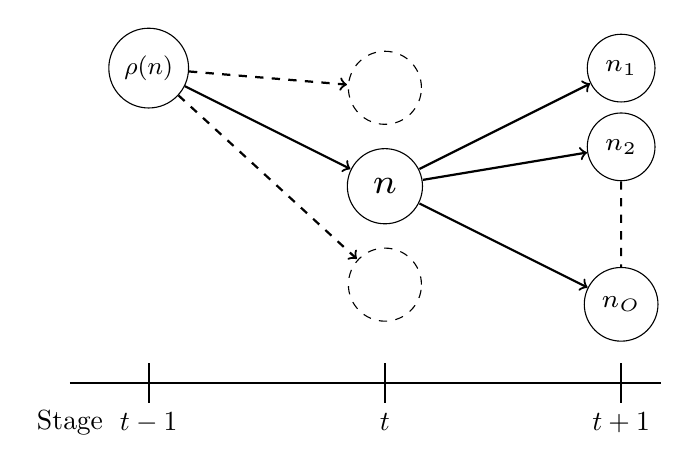
\begin{tikzpicture}

\draw (-1,2.5) node(RHO)[circle,draw]{\small $\rho(n)$ };
\draw (2,2.25) node(NUP)[circle,dashed,scale=2.8,draw]{ };
\draw (2,1) node(N)[circle,scale=1.8,draw]{\scriptsize $n$ };
\draw (2,-.25) node(NDOWN)[circle,dashed,scale=2.8,draw]{ };
\draw (5,2.5) node(N1)[circle,scale=1.3,draw]{\scriptsize $n_1$ };
\draw (5,1.5) node(N2)[circle,scale=1.3,draw]{\scriptsize $n_2$ };
\draw (5,-.5) node(NO)[circle,scale=1.3,draw]{\scriptsize $n_O$ };

\draw[thick,dashed, ->] (RHO) -- (NUP);
\draw[thick,->] (RHO) -- (N);
\draw[thick,dashed, ->] (RHO) -- (NDOWN);
\draw[thick,->] (N) -- (N1);
\draw[thick,->] (N) -- (N2);
\draw[thick,->] (N) -- (NO);
\draw[thick,dashed] (N2) -- (NO);

\draw[thick] (-2,-1.5) -- (5.5,-1.5);
\draw[thick] (-1, -1.75) -- (-1, -1.25);
\draw[thick] (2, -1.75) -- (2, -1.25);
\draw[thick] (5, -1.75) -- (5, -1.25);

\draw(-2,-2) node {Stage};
\draw(-1,-2) node {$t-1$};
\draw(2,-2) node {$t$};
\draw(5,-2) node {$t+1$};

\end{tikzpicture} 
\caption{Stochastic tree for Mixed-Integer Formulation}
  \label{fig:mip}
\end{figure}


\subsection{Decision Dependent Uncertainty}
In order to model the decision dependent uncertainty, a cumulative distribution function (cdf) for line failures based on loaded is needed.  This model uses a parameter, $R$, to represent the effective capacity of a line.  This is found by sampling from the cdf before formulating the problem.  This effective capacity represents the loading of the transmission line that will cause its failure.  This failure is represented in the binary variable, $z$. \\

In Mixed-Integer Programming, there have been standard equations developed to model logical conditions.  This problem has two logical conditions that need to be modeled in order to represent this decision dependent uncertainty.  First, the condition that the line will fail if it has more power flow than its effective capacity.
\begin{align*}
\mbox{If }
		\hspace{30px}&\left| f_{e\rho(n)} \right| > R_{en}  \\
\mbox{Then }
		\hspace{30px}&z_{en} = 0
\end{align*}

To model this logic, a Big-M constraint can be used, where M represents a large number.
\begin{align}
	f_{e\rho(n)} - R_{en} &\le M^R_e (1-z_{en})	\label{r1}\\
	f_{e\rho(n)} + R_{en} &\ge - M^R_e (1-z_{en})	\label{r2}
\end{align}
with $M^R_e = U_e - R_e$. \\

Now, when the line is available in stage $n$, that is $z_{en} = 1$, then the line flow in the predecessor node is within the effective capacity, -$R_{en} \le f_{e\rho(n)} \le R_{en}$.		\\

The second logical condition is that when the line is unavailable, the power flow on that branch is zero and the phase angles between the two nodes are not constrained. 
\begin{align*}
\mbox{If }
		\hspace{20px}&z_{en} = 0	\\
\mbox{Then }
		\hspace{20px}&f_{en} = 0  \hspace{10px} \mbox{ and}\\
				&\theta_{in} - \theta_{jn} - X_{e}f_{en} \mbox{ is arbitrary}
\end{align*}	

This can be achieved through the following equations.
\begin{align}
-U_{e} z_{en} \le f_{en} &\le U_{e} z_{en}	\label{lf1}\\
\theta_{in} - \theta_{jn} + X_e f_{en} &\ge -M^\theta_e(1-z_{en}) \label{lf2} \\
\theta_{in} - \theta_{jn} + X_e f_{en} &\le M^\theta_e(1-z_{en})  \label{lf3}
\end{align}
with $M^\theta_e = 2 \theta_{max} + X_e U_e$.

\subsection{Sampling}
The OPA simulation uses a step function for the failure probability of a line.  A line will fail if it $f_e \ge \alpha U_e$ with probability $p$.    To model that scenario here, a sample from the distribution can be used to form the effective capacity of the lines.  Let $\omega_n \equiv\left[ 0, 0, 1, 0, \cdots, 1\right]$  be a vector sampled from the probability distribution.  Now, a line will fail if $f_e \ge \alpha U_e$ and $w_{ne} =1$.  With this sampling, the effective capacity can be designed to incorporate this information.    
\begin{equation}
 R_{ne} = 
 \left\{ 
	\begin{array}{lr}
				\alpha U_e & \mbox{if } \omega_{ne}=1\\
			  U_e + \epsilon & \mbox{if } \omega_{ne}=0
	\end{array}
 \right. \label{r}
\end{equation}

The resulting set of effective capacities $R$ can be represented by a cumulative distribution function. The distribution in Figure \ref{cdf} is one example of a viable line failure distribution input.  It is the result of a uniform distribution for $\alpha$ between $L$ and 1 and Bernoulli trial with probability $p$ for $\omega$.  


\pgfplotsset{every axis plot/.append style={line width=2pt}}
\tikzset{
every pin/.style={fill=yellow!50!white,rectangle,rounded corners=3pt,font=\tiny},
small dot/.style={fill=black,circle,scale=0.3}
}
\begin{figure}
\centering
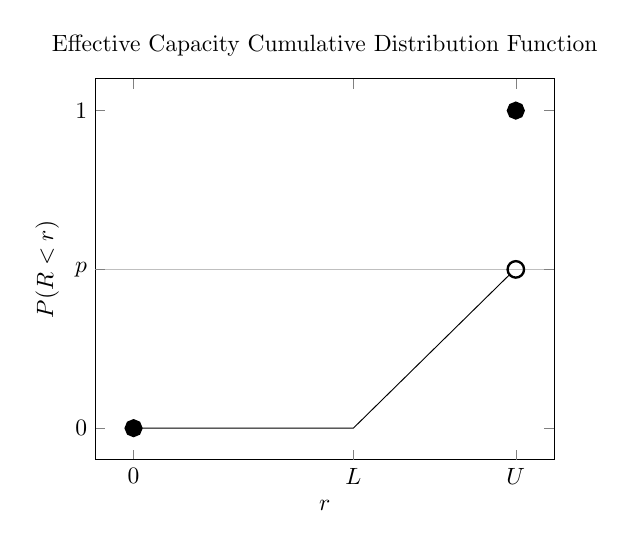
\begin{tikzpicture}[scale=.85]
\begin{axis}[ 
	xlabel=$r$,
	ylabel=$P( R < r )$,
	title = Effective Capacity Cumulative Distribution Function,
	unbounded coords = jump,
	xtick= {0},
	ytick= {0, 1},
	extra y ticks={.5},
	extra y tick style={grid=major},
	extra y tick labels={$p$},
	extra x ticks={.575,1},
	extra x tick labels={$L$, $U$},
scatter/classes={
 		 a={mark=o,line width=3.5pt},%
 		 b={mark=o,line width=1pt,scale=1.75}%
		}]
	\addplot[black] coordinates { 
		(0,0)		
		(.575,0)	
		(.985,.485) 		
		(1,inf)		
		(1,1)		
		};	
	\addplot[ 
		scatter,only marks,
		scatter src=explicit symbolic]
		coordinates {  
		(0,0)		[a]
		(1,.5)		[b]
		(1,1)		[a]
		};


	

\end{axis}
\end{tikzpicture}

\caption{ Example Effective Capacity Distribution for equation (\ref{r}) }
\label{cdf}
\end{figure}



\subsection{Feasible Cascades}
The cascading process begins with an intial exogenous event, $\xi \in \left\{ 0, 1 \right\}^{\magE}$.  The following equation enforces a line outage throughout the whole cascade for all $\xi = 1$.

\begin{equation}
z_{en} \le 1- \xi_e  \label{xi}
\end{equation}

Now, the set of all feasible cascades can be described as follows, 
\begin{equation}
\cX(\xi) \equiv \left\{ \left(d, p, f, z \right)  |  \mbox{ \cref{pf1,pf2,r1,r2,lf1,lf2,lf3,r,xi}  hold } \right\} 
\end{equation}
where $d = \left[ d_0, d_1, \cdots, d_N \right]$ is the set of vectors of demand served for each node in the scenario tree.  Now, this compact representation of the cascading process can be used in many ways.  One way is a chance constrained model, in which the operator requires a line to be available in a certain percentage of scenarios.  Another way is to use this as a subproblem in a larger planning model. 

\subsection{Least Cost Dispatch}
The following model is a least cost dispatch model that includes the effects from cascading failures due to a set of contingencies $\xi\in\Xi$.  
\begin{subequations}
\label{leastcost}
\begin{align} \displaystyle
	{\large \mbox{min}} \hspace{10px} &  \Expect_\Xi \sum_{in} \left[ C_{in}  p_{in,m}  + W_{in} (\hat{d}_{i} - d_{in,m}) \right]	\\
	&(d,p,f,z)_m  \in \cX(\xi_m)    \hspace{20px}   \forall \xi_m \in \Xi	
\end{align}
This can be adapted to several different problems in power systems.  The main difficulty with this multi stage stochastic program is computational complexity.  In order to find an appropriate size for the number of outcomes and stages in the model, a calibration routine will be used to find a set of parameters in which the MSIP model is similar to the OPA model.
\end{subequations}


\subsection{Model Calibration}
In order to get reliable output from the optimization routine, this model needs to be calibrated against the OPA simulation.  The primary calibration parameters are $L$ and $p$ in the line failure distribution as well as the costs for load shed, $W$, which depend upon the stage in the cascade.  The OPA simulation is a greedy algorithm, attempting to maximize demand served in the current stage without regard to the line failure consequences.  In order to capture this effect, more weight was placed on demand served in earlier stages of the cascade. \\

 The root problem used is comprised of 4 intitial outages and each outage has a scenario tree that is 4 stages long with 2 outcomes at each node.  The power system modeled is the IEEE 118 bus grid with a nominal demand of 3668 MW and around 29,600 MW in branch capacities.  The parameters choosen for the MSIP model were $p=.5$, $L =.575$.  The weight for the stages of the cascade were $[500, 10, .05, .0001]$, which seemed to capture the greedy behavior of the OPA simulation.  The OPA simulation used the step function failure model with $\alpha=.99$ and $p=.5$.  The output of the simulation and MSIP formulation are shown in Table (\ref{compare}) along with the load shed distribution for $\xi = [12,14,34,111]$ in Figure (\ref{dist}). 


% Calibrate ---------------------------------------------------------


\begin{figure}
 \centering
	\begin{tikzpicture}
		\begin{axis}[xlabel=$LS$ (MW), ylabel=$P($Load Shed $> LS )$
				,legend pos=north east
				,grid=major,
				,xmin=-25,xmax=400
				,title=\mbox{Load Shed Distribution} ]


 	\addplot[black,line width=3pt] table[x=mv, y=mp] {./data/calibrate.txt};
	\addlegendentry{MSIP}
	
	\addplot[red,line width=2pt] table[x=sv, y=sp,mark=square] {./data/calibrate.txt};
	\addlegendentry{SIM}





		\end{axis}	
	\end{tikzpicture}
  \caption{Load Shed Distribution for the OPA simulation and MSIP formulation}
 \label{dist}
\end{figure}





\begin{table}
\centering
\begin{tabular}{| c | c c | c c |}
\hline
	&	\multicolumn{2}{ | c | }{ SIM } & \multicolumn{2}{|c|}{MSIP} \\
$\xi$ 	&	$\Expect [ LS ]$ & St.Dv.$ [LS]$ &	$\Expect [LS]$ & St.Dv.$ [LS]$  \\
\hline
\hline
2,12,21 &	196 & 128.1 & 184 & 112.7 \\
5,25,34, 82 &	254 & 187.1 & 160 & 69.3 \\
12,14,34,111 & 	131 &	 85.12 &	 151 &	 59.0 \\
13,24 	&	145 & 123.4 	&	123	&	84.4 \\

\hline
\end{tabular}
\caption{Comparison of Simulation and MSIP outputs}
\label{compare}
\end{table}

%
\begin{figure}
\centering

\begin{tikzpicture}[scale=1]
	\begin{axis}[
x tick label style={
/pgf/number format/1000 sep=},
ylabel=Population,
enlargelimits=0.05,
legend style={at={(0.5,-0.15)},
anchor=north,legend columns=-1},
ybar interval=0.7,
]
%[ybar, xlabel=Line, ylabel=Outages, title=\mbox{\textbf{ Outages by Line Number }} ]


\foreach \i in {2,4,8,16,32,64,128}
{
	\addplot[ bar width=0em] table[x=line, y=outages ]{./data/lineOutage_\i.out};
	\addlegendentryexpanded{\i x}
}
	\end{axis}
\end{tikzpicture}
\caption{Line Outage thing}

\end{figure}



\section{Model Flexibility}
The primary strength of this formulation is the flexibility it has in using additional constraints and objectives to inform decision making about power systems.  All of these models can then be solved with commercial solver software without the need to develop additional specialized routines.  This paper will develop the models for 4 different problems currently in the power systems field and provide a computation example of one of them.  The first model will be a chance constrained model, which enforces a probablistic constraint on the number of line outages in any scenario.  The second model will be a redispatch model that moves to a generator configuration that is close to the original while minimize the expected size of the cascade.  The third model will be a reserve planning model that allocates reserves among the generators in such a way as to minimize the worst case failure.  Finally, a transmission expansion model will be developed that allocates a budget for capacity expansion on the grid in such a way as to minimize the expected size of the cascade.  This example will have computation results and compare them with the OPA simulation to a simple heuristic which allocates the expansion budget.
\subsection{Chance Constraint on N-k Criteria}
In this model, constraints are used to express the probability that less than a given number of lines are outaged is close to 1.  A typical case in power systems would be that the system should not go beyond 1 contingency in a large percentage of scenarioes.
\begin{equation}
P\left\{\text{Line Outage} \le k \right\} \ge 1 - \epsilon
\end{equation}
This can be done by adding another binary variable for each scenario that represents whether or not that scenario has less than $k$ outages.  Then these new binary variables will be summed and constrained by the given probability.
\begin{subequations}
\begin{align}
\sum_i z_{is} &\le	M_s \hat{z_s} + | \xi_s | + k \\
\sum_s \hat{z_s} &\le \epsilon | \cS |
\end{align}
\end{subequations}
where $M_s = | \cE | - | \xi_s | - k$.  The objective of this program would be to minimize load shed as in (\ref{leastcost}) such that the power system does not lose more than $k$ branches.
\subsection{Generator Redispatch}
This model tries to find a operating configuration that is within a given distance from the current operating regime and minimizes the worst case scenario outage.  The input for this model is the current operating configuration $(p_0, d_0)$ as well as a distance vector $\delta$ that represents how far each generator can move from its current output levels.  In this case, the root node of the stochastic tree will have variables that represent initial generator output levels and the child trees will be constrained from how far they can move from this.  Also, a continuous variable will be added that represents the amount of load shed in the worst case scenario.  The objective will be to minimize this worst case scenario.  
\begin{equation}
p - p_0 \le \delta
\end{equation}
\begin{equation}
l \ge \sum_i \hat{d}_i - d_{is}
\end{equation}
aim to min 
This program could be used when the system is becoming close to unstable and cost concernes become less of a priority than system stability.


\subsection{Operating Reserves}
In this case an operating configuration need not be given.  The program can either search for an operating configuration as well as reserves or given an operating configuration, allocate the reserves.  These operating reserves determine where the system is able to relieve congestion in a contingency.
\begin{align}
p_{in} + r_{in} &\le \overline{P}_i \\
p_{in} &\le p_{i\rho (n)} + r_{i\rho (n)} \\
\sum_i r_{in} &\le \beta \sum_i \hat{d}_i 
\end{align}
where $\beta$ is the level of operating reserves allotted for the system.

\section{Transmission Expansion}
Using the MIP formulation, a stochastic program can be developed to model planning decisions with respect to cascading power failures.  Consider the problem of transmission expansion.  A set of contingenciences, $\xi \in \Xi$, has been identified as the primary risk for initiating a cascading event.  There is a budget to use for expansion and the objective is to allocate the budget in such a way as to minimze some risk measure of load shed for the cascading power failures. \\

Let $x$ be the design variable, which is decided at the root node and represents additional capacity on power lines.  This affects the constraint set such that equations (\ref{lf1}) and (\ref{r}) become  
\begin{align}
-(U_{e}+x_e) z_{en} \le f_{en} \le (U_{e}+x_e) z_{en} &	\label{lfm}	\\
 R_{ne} = 
 \left\{ 
	\begin{array}{lr}
				\alpha (U_e + x_e) & \mbox{if } \omega_{ne}=1\\
			  (U_e + x_e) + \epsilon & \mbox{if } \omega_{ne}=0
	\end{array}
 \right. \label{rm}
\end{align}



\begin{figure}
\centering
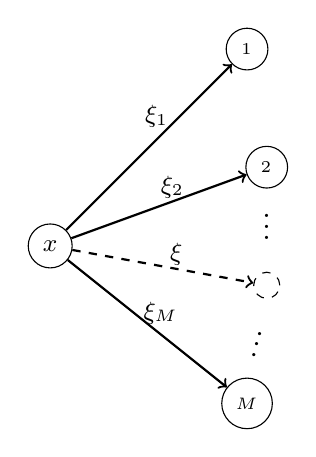
\begin{tikzpicture}

\draw (.5,.5) node(ROOT)[circle,draw]{\small $x$ };
\draw (3,3) node(ONE)[circle,draw]{ \small $\cX_1$ };
\draw (3.25,1.5) node(TWO)[circle,draw]{ \small $\cX_2$ };
\draw (3.25,.85) node(DOTONE){ \large $\vdots$ };
\draw (3.25,0) node(N)[circle,dashed,draw]{ \small $\cX$ };
\draw (3.15,-.65) node(DOTTWO)[rotate=-15]{ \large $\vdots$ };
\draw (3,-1.5) node(S)[circle,draw]{ \small $\cX_M$ };

\draw (1.85,2.15) node(OMG1){ \small $\xi_1$ };
\draw (2.05,1.25) node(OMG2){ \small $\xi_2$ };
\draw (2.1,.4) node(OMG){ \small $\xi$ };
\draw (1.9,-.35) node(OMGS){ \small $\xi_M$ };

\draw[thick, ->] (ROOT) -- (ONE) ;
\draw[thick,->] (ROOT) -- (TWO);
\draw[thick,dashed, ->] (ROOT) -- (N);
\draw[thick,->] (ROOT) -- (S);

%\draw[thick,dashed] (TWO) -- (N);
%\draw[thick,dashed] (N) -- (S);

\end{tikzpicture} 
\caption{Scenario Tree for Two Stage Problem}
  \label{fig:mip}
\end{figure}



The objective is to allocate a budget for capacity additions in order to reduce the expected blackout size.  $W_{in}$ is the cost of load shed at bus $i$ in node $n$ of the scenario tree.  $B$ is the budget for capacity expansion.
\begin{subequations}

\begin{align} \displaystyle
	{\large \mbox{min}} \hspace{10px} &  \Expect_\Xi \sum_{in} \left[ C_{in}  p_{in,m}  + W_{in} (\hat{d}_{i} - d_{in,m}) \right]	\\
	&(d,p,f,z)_m  \in \cX(\xi_m)    \hspace{20px}   \forall \xi_m \in \Xi	\\
	& \underline{X}_e y_e \le x_e \le \overline{X}_e y_e \hspace{35px} \forall e \in \cE\\
	&\sum_e x_e \le B_x 	\\
	& \sum_e y_e \le B_y  
\end{align}
\label{TX}
\end{subequations}



\subsection{Computational Results}
The model outlined in (\ref{TX}) is solved using Gurobi 4.5.  The stopping criteria was either a 40\% optimality gap or 10,000s.  The program was run for several different expansion budgets, with both the total budget and the maximum number of lines being changed.  The output of this model is a vector $x$ which represents the amount of capacity to add to each power line on the grid.  This is used to modify the initial grid and run the OPA simulation to find the effects it has on the system.  In order to find out whether these solutions are reasonable or not, a heuristic was developed to compare against.

\subsubsection{Heuristic}
The heuristic used is based on a large number of OPA simulation runs in which the power lines were ranked in descending order based on the percentage of runs in which that given power line was outaged.  Then, for a given total budget $B_x$ and maximum number of changed lines $B_y$, the heuristic picks the top $B_y$ lines in the list and then distributes the budget $B_x$ evenly over the lines.

\subsection{Comparing Results}
The OPA simulation is used to compare the results of the two models.  Since the MSIP was calibrated based on the 4 contingencies, a second set of OPA simulation was used with 4 random initial contingencies to start the cascade.




\begin{figure}
 \centering
	\begin{tikzpicture}
		\begin{axis}[xlabel=$LS$ (MW), ylabel=$P($Load Shed $> LS )$
				,legend pos=north east
				,grid=major,
				,xmin=-25,xmax=1300
				,title=\mbox{Load Shed Distribution} ]


 	\addplot[red,line width=2pt] table[x=ls, y=prob] {./data/d25k20.dat};
	\addlegendentry{design}
	
	\addplot[blue,line width=2pt] table[x=ls, y=prob,mark=square] {./data/dumb25k20.dat};
	\addlegendentry{heuristic}

	\addplot[black,line width=2pt] table[x=ls, y=prob,mark=square] {./data/sim.dat};
	\addlegendentry{nom}




		\end{axis}	
	\end{tikzpicture}
  \caption{Load Shed Distribution for the OPA simulation and MSIP formulation}
 \label{dist}
\end{figure}

% Calibrate ---------------------------------------------------------

\subsection{Conclusion}
Using the OPA simulation as a reference for how the grid may respond to cascading power failures, a mixed integer model was developed which represents the cascading effects over a fixed number of outcomes and stages.  While this model can be difficult computationally due to the decision dependent uncertainty, it is extremely flexible.  The model can be used to include cascading effects in a wide range of power system problems with optimality criteria ranging from least cost to minimize worst case problems.  A computation example was done on transmission expansion, which showed the model was able to better than a reasonable heuristic, even though it was only solved to a 40\% optimality gap.  Future work can be done in order to improve the solve time for these types of models based on techniques developed in stochastic and mixed integer optimization.

